The reason the progressive GAN is not featured in these results can be seen in figure \ref{fig:fadeVsFreeze}.

A comparison between a VAE and the autoencoder part of an AEGAN is shown in figure <Referera till figur>. It is clear from this illustration that the simultaneous training of the GAN caused the autoencoder to generate more visually pleasing samples.

Quantitative results can be seen in table \ref{tab:quantitative_results}.

\begin{figure}[t]
    \centering
    \begin{subfigure}[b]{0.49\textwidth}
        \includegraphics[width=\textwidth]{results/freezeInDG1_2.eps}
        \caption{Weight freezing in old layers}
        \label{fig:freezeInDG1}
    \end{subfigure}
    \begin{subfigure}[b]{0.49\textwidth}
        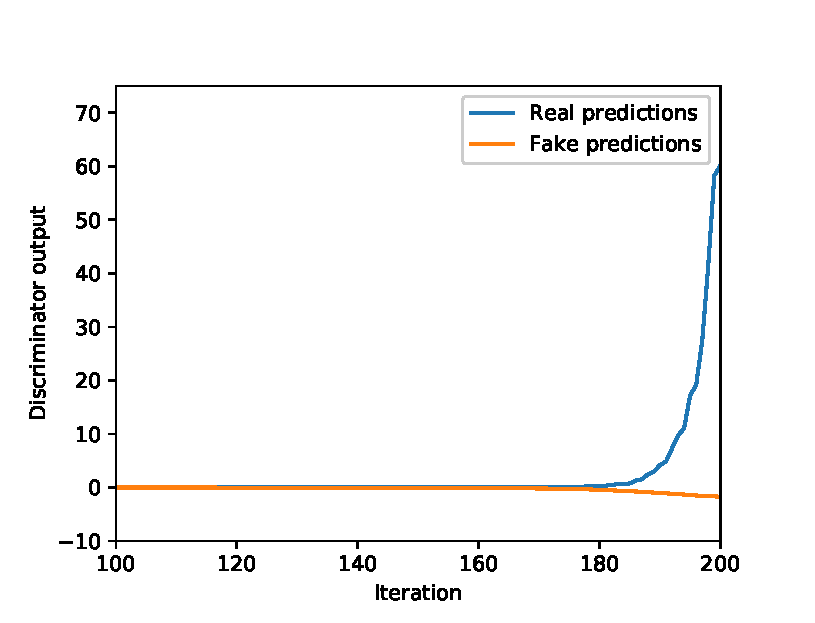
\includegraphics[width=\textwidth]{results/fadeInDG1_2.eps}
        \caption{Fade in new layers}
        \label{fig:freezeInDG2}
    \end{subfigure}
    \caption{Discriminator output on real and fake images during transition between 16x16 and 32x32 resolution images for the different transition strategies on the synthetic data se.}
    \label{fig:fadeVsFreeze}
\end{figure}

\begin{table}[t]
    \centering
    \caption{Jaccard distance between recognized }
    \label{tab:quantitative_results}
    \begin{tabular}{l|l|l}
    \hline
    %\multicolumn{3}{c}{Generator}           \\ 
    Training data type      & MEE synthetic data  & MEE Accuracy real data \\ \hline
    Original data           & $\sim$ 0.3 & 1.1     \\
    VAE                     & $\sim$ 1.7 & 1.9     \\
    VAE + original data     & 0.3 (guess) & 134     \\
    %PGAN                    & 5.4 (pessimistic guess) & 134     \\
    %PGAN + original data    & 0.3 (optimistic guess) & 134     \\
    AEGAN                   & 0.3 (optimistic guess) & 134     \\
    AEGAN + original data   & 0.3 (guess) & 134     \\
    \end{tabular}
\end{table}

\begin{table}[t]
    \centering
    \caption{Number of iterations of training for the different algorithms}
    \label{tab:quantitative_results}
    \begin{tabular}{l|l|l}
    \hline
    %\multicolumn{3}{c}{Generator}           \\ 
    Training data type      & Synthetic data  & Real data \\ \hline
    VAE                     & 560000 & 560000 \\
    PGAN                    & idk & idk     \\
    AEGAN                   & 520000 & 840000   \\
    \end{tabular}
\end{table}

TODO: Visa kapacitet/overfitting på samma dataset, visa att genererad data är konsistent och har bra annoteringar!

<<Lägg till ett par histogram här.>>
